\documentclass[conference]{IEEEtran}

\usepackage[T1]{fontenc}
\usepackage[utf8]{inputenc}
\usepackage{cite}
\usepackage{graphicx}
\usepackage{booktabs}
\usepackage{url}
\usepackage{listings}
\usepackage{xcolor}

\lstset{
  basicstyle=\ttfamily\scriptsize,
  breaklines=true,
  columns=fullflexible,
  frame=single,
  backgroundcolor=\color[gray]{0.96}
}

\title{Beyond CPU-Based Horizontal Pod Autoscaling: Empirical Limits of Kubernetes Autoscaling in Local and Managed Cloud Environments}

\author{\IEEEauthorblockN{Ivo Motoki Makiyama Lopes}
\IEEEauthorblockA{Escola Politecnica, Universidade de Sao Paulo\\
PSI5120 -- Topicos de Computacao em Nuvem\\
ivo.motoki@usp.br\\
\url{https://github.com/IvoMotoki/psi5120-trabalho-hpa}}}

\begin{document}
\maketitle

\begin{abstract}
Horizontal Pod Autoscaling (HPA) is a central mechanism for elastic cloud-native applications, but increasing the desired number of replicas does not guarantee that a cluster can actually schedule and run them. This paper extends a previous Kubernetes HPA experiment by comparing the same CPU-bound web workload in local Minikube and managed Amazon EKS environments, then adding an HPA behavior-tuning experiment. The study measures reaction time, time to peak replicas, scale-down delay, effective schedulable capacity, and replica-seconds as an operational cost proxy. The baseline Minikube run reached the configured maximum of 10 replicas without pending workload pods. In contrast, the EKS runs were capped at 5 desired replicas and showed up to 4 pending workload pods, exposing the effect of node-level pod density and Amazon VPC CNI constraints. In the additional Minikube tuning experiment, a fast scale-down policy reduced replica-seconds by 25.7\% relative to a comparable baseline rerun. The paper argues that practical elasticity requires reasoning about the metrics pipeline, HPA policy, scheduler capacity, node autoscaling, and cloud cost together.
\end{abstract}

\begin{IEEEkeywords}
Kubernetes, Horizontal Pod Autoscaler, Amazon EKS, Minikube, cloud computing, autoscaling, container orchestration.
\end{IEEEkeywords}

\section{Introduction}

Autoscaling is one of the main operational promises of cloud computing: instead of provisioning fixed capacity for peak demand, applications can adapt resource allocation to observed load. In Kubernetes, the Horizontal Pod Autoscaler (HPA) implements this mechanism by periodically changing the replica count of scalable workloads such as Deployments based on metrics such as CPU utilization~\cite{kubernetes_hpa_concepts}.

In practice, however, HPA is only one control loop inside a larger system. It can request more replicas, but it cannot by itself guarantee that the cluster has enough schedulable capacity, IP addresses, node resources, or cloud budget to run them. This distinction is especially important in managed Kubernetes environments such as Amazon EKS, where pod density depends not only on CPU and memory but also on instance type and Amazon VPC CNI networking limits~\cite{aws_eks_vpc_cni}.

This distinction matters pedagogically and operationally. In an introductory experiment, it is tempting to interpret the HPA object as the autoscaling system. In production, the actual system includes resource requests and limits, Metrics Server, the HPA controller, the Kubernetes scheduler, node capacity, networking limits, and often a separate node autoscaler. If any of these layers is missing or constrained, the application may remain underprovisioned even when the HPA policy is syntactically correct.

This work extends an intermediate PSI5120 project that deployed the official Kubernetes CPU-bound HPA example workload in both Minikube and Amazon EKS. The final project has three goals: first, to quantify the baseline behavior already observed in both environments; second, to add a controlled experiment using explicit \texttt{autoscaling/v2} behavior policies; and third, to analyze why effective elasticity in EKS can be bounded by infrastructure constraints outside the HPA object itself. The contribution is intentionally empirical and reproducible: the paper does not propose a new autoscaling algorithm, but it turns a course experiment into a compact study of where Kubernetes autoscaling succeeds, where it stops, and which evidence should be collected to diagnose that boundary.

The guiding research questions are:

\begin{itemize}
  \item RQ1: With the same workload and HPA target, how do Minikube and EKS differ in reaction time, peak replicas, and scale-down behavior?
  \item RQ2: When HPA recommends additional replicas in EKS, which infrastructure limits can prevent those replicas from becoming ready?
  \item RQ3: How do explicit HPA behavior policies change underprovisioning and overprovisioning windows compared with Kubernetes defaults?
\end{itemize}

\section{Background}

\subsection{Horizontal Pod Autoscaler}

The Kubernetes HPA controller periodically computes a desired replica count from observed metrics. For resource metrics such as CPU, the controller compares current utilization with the configured target and conceptually applies the ratio between the current and desired values~\cite{kubernetes_hpa_concepts}. CPU utilization is expressed relative to each container's \texttt{resources.requests.cpu}, so missing or poorly chosen requests can make HPA behavior undefined or misleading.

The core proportional rule can be written with compact notation as:

\begin{equation}
D = \left\lceil R \times \frac{M_c}{M_t} \right\rceil .
\end{equation}

In the equation, \(D\) is the desired replica count, \(R\) is the current replica count, \(M_c\) is the current metric value, and \(M_t\) is the target metric value.

This simple expression hides several practical details. Pods that are not yet ready or that do not have usable metrics may be treated specially by the controller. With multiple metrics, Kubernetes computes one recommendation per metric and uses the largest desired replica count. The controller also avoids reacting to very small metric changes through tolerance rules~\cite{kubernetes_hpa_concepts}. Therefore, observed behavior should be interpreted as the output of a control loop, not as an instantaneous arithmetic operation.

The default HPA control loop favors fast scale-up and conservative scale-down. Kubernetes documents a default 15 s synchronization period for the controller and a default 300 s stabilization window for scale-down recommendations~\cite{kubernetes_hpa_concepts}. The \texttt{autoscaling/v2} API exposes a \texttt{behavior} field that allows experiments with explicit scale-up and scale-down policies, including stabilization windows, pod-based policies, percent-based policies, and policy selection rules~\cite{kubernetes_hpa_api_v2}. This field is the basis of the tuning experiment in this paper.

\subsection{Metrics Pipeline}

The HPA does not collect resource metrics directly. It relies on the Kubernetes metrics APIs, commonly backed by Metrics Server. Metrics Server is intended as an efficient source for autoscaling resource metrics, not as a general-purpose monitoring or historical observability system~\cite{kubernetes_metrics_server}. This distinction motivates the use of experiment logs and derived CSV data in this project.

The implication is important for measurement design. The values seen through \texttt{kubectl get hpa} and \texttt{kubectl top pods} are sufficient to explain HPA decisions, but they are not a high-resolution performance trace. For that reason, this study reports control-loop metrics such as time to first scale-up, time to peak replicas, scale-down delay, pending pods, and replica-seconds. It does not claim request-level latency or throughput results.

\subsection{Amazon EKS Capacity Constraints}

Amazon EKS runs standard Kubernetes HPA behavior, provided that a metrics source such as Metrics Server is available~\cite{aws_eks_hpa}. The managed cloud environment adds other constraints. With the Amazon VPC CNI plugin in the default mode, pods receive VPC IP addresses, and pod density is bounded by the number of elastic network interfaces and IP addresses supported by each EC2 instance type~\cite{aws_eks_vpc_cni}. Therefore, a workload may hit scheduling limits even when the HPA \texttt{maxReplicas} value is higher.

This paper uses the term \emph{configured elasticity} for the desired range expressed in the HPA object, such as \texttt{minReplicas: 1} and \texttt{maxReplicas: 10}. It uses \emph{effective elasticity} for the replicas that can actually be scheduled and become useful. The gap between these two values is the main difference observed in EKS.

\section{Related Work}

Recent work has evaluated HPA in microservice environments, including throughput, latency, resource utilization, and operational cost trade-offs~\cite{buzato_goldman_2026_hpa}. Other studies have proposed finer-grained horizontal scaling policies to address delayed response and conservative anti-oscillation behavior in container clouds~\cite{jiang_wu_2021_fine_grained_hpa}. This paper is narrower in workload complexity, but contributes a reproducible educational comparison between a local Kubernetes cluster and a managed cloud cluster under realistic infrastructure limits.

The scope also differs from work on proactive or event-driven autoscaling. This study focuses on reactive CPU-based HPA because it is the default learning path in Kubernetes and EKS documentation~\cite{kubernetes_hpa_walkthrough,aws_eks_hpa}. Event-driven techniques, external metrics, KEDA, Cluster Autoscaler, and Karpenter are discussed as extensions, but they are not the primary experimental object. This keeps the experiment small enough to reproduce while still exposing the layered nature of cloud elasticity.

\section{Experimental Setup}

\subsection{Environments}

The local environment is a Minikube cluster running in WSL2 on a Windows host. The cluster uses a single node profile named \texttt{hpa-2026}, with 4 virtual CPUs and 6144 MB of memory allocated during the final reruns. Metrics Server is enabled through the Minikube addon mechanism, and all workload resources run in a dedicated namespace named \texttt{tf-hpa}.

The cloud environment is Amazon EKS in \texttt{us-east-1}, created with \texttt{eksctl}. The intermediate experiment used a managed node group based on \texttt{t3.micro} instances. This instance type was selected because the AWS account used for the course constrained EC2 usage to Free-Tier-eligible instances. The constraint is useful for the final analysis because it makes the difference between HPA configuration and schedulable capacity visible.

\subsection{Workload}

Both environments run the official Kubernetes HPA walkthrough workload, \texttt{registry.k8s.io/hpa-example}, exposed through a \texttt{php-apache} Deployment and Service~\cite{kubernetes_hpa_walkthrough}. The container requests 200 mCPU and 64 MiB of memory, with limits of 500 mCPU and 128 MiB. The baseline HPA targets 50\% average CPU utilization with \texttt{minReplicas: 1} and \texttt{maxReplicas: 10}.

The use of the official CPU-bound example is deliberate. It avoids introducing an application-specific bottleneck and aligns the course experiment with the Kubernetes and EKS documentation. The workload is not intended to model a complete web application; it is a controlled actuator for the HPA loop.

\subsection{Load Generation}

Load is generated from inside the cluster using BusyBox pods repeatedly issuing HTTP requests to the internal Kubernetes Service DNS name:

\begin{lstlisting}
while true; do
  wget -q -O- http://php-apache.tf-hpa.svc.cluster.local
done
\end{lstlisting}

This avoids differences caused by external network exposure and keeps the stress method comparable between Minikube and EKS. The final Minikube tuning runs used six generator pods, 240 s of active load, and a 720 s post-load window. The longer post-load window was chosen to capture the default scale-down stabilization behavior, which can outlive a short observation window.

\subsection{Measurements}

The experiment logs \texttt{kubectl get hpa}, \texttt{kubectl get pods -o wide}, and \texttt{kubectl top pods} during active load and after load removal. The final project derives the following metrics from raw logs: time to first scale-up, time to peak replicas, time to scale-down, peak desired replicas, running workload pods, pending workload pods, replica-seconds, and time spent above the CPU target.

Replica-seconds are computed by multiplying the HPA desired replica count observed in each interval by the interval duration and summing across the run. This is not a monetary cost by itself, but it is a useful proxy for provisioned application capacity. A policy that holds more replicas for longer has a higher replica-second value and would tend to consume more resources in a cluster with sufficient node capacity.

\subsection{Reproducibility}

The project stores raw logs, derived CSV files, generated tables, figures, HPA manifests, and parsing scripts. Raw logs are kept under \texttt{evidencias/}, while final-project artifacts are kept under \texttt{final-ieee/}. The parser accepts HPA samples with both numeric CPU values and transient \texttt{<unknown>} CPU values, preserving replica counts even before Metrics Server reports a usable target. This matters because the first samples of a fresh run may have undefined CPU metrics while the workload is already running.

\section{Baseline Results}

The baseline analysis uses the raw timeline logs produced in the intermediate project. Each run records HPA state, pod state, and resource metrics during the active-load window and after load removal. Table~\ref{tab:baseline-generated} summarizes the metrics extracted automatically from those logs.

\begin{table}[ht]
\centering
\caption{Baseline HPA metrics extracted from raw experiment logs}
\label{tab:baseline-generated}
\resizebox{\linewidth}{!}{%
\begin{tabular}{lrrrrr}
\toprule
Run & First scale-up (s) & Peak replicas & Pending pods & Scale-down after load (s) & Replica-s \\
\midrule
Minikube baseline & 82 & 10 & 0 & 144 & 2450 \\
EKS baseline 005559 & 230 & 5 & 4 & -- & 1983 \\
EKS baseline 010657 & 50 & 5 & 4 & 351 & 2773 \\
\bottomrule
\end{tabular}
}
\end{table}


\begin{figure}[ht]
\centering
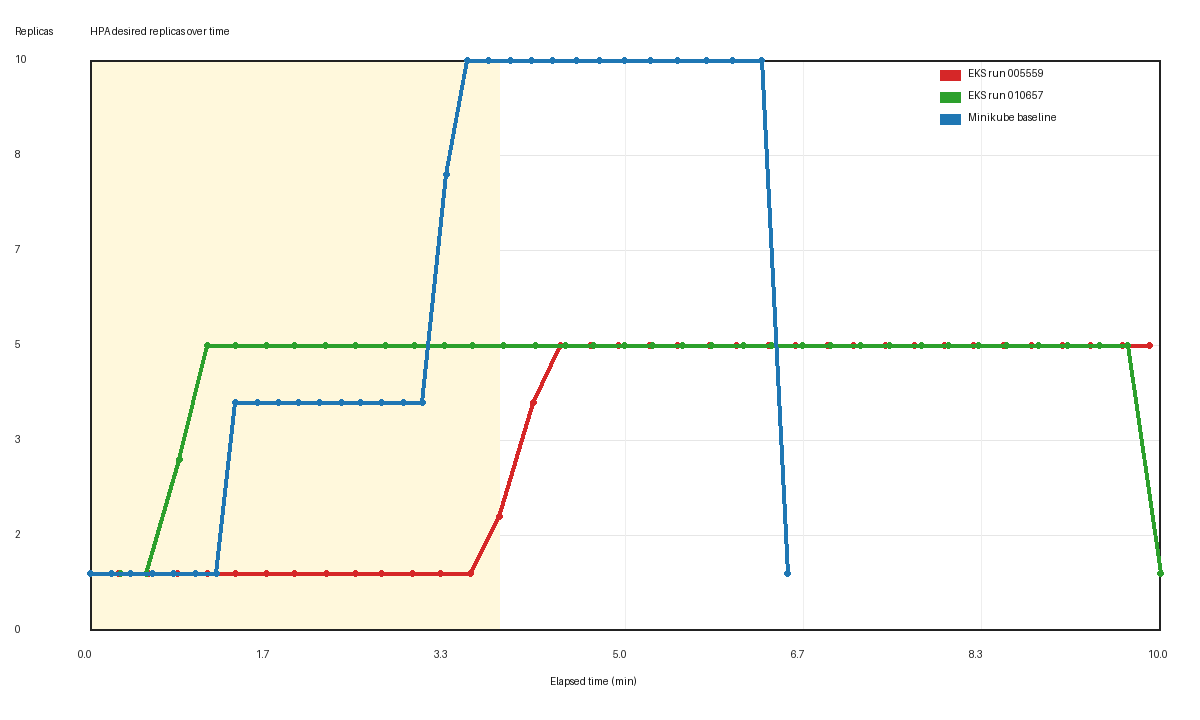
\includegraphics[width=\linewidth]{figures/baseline_hpa_replicas.png}
\caption{HPA desired replicas over time for the existing baseline runs. The shaded area indicates the active-load phase of the first parsed run.}
\label{fig:baseline-hpa-replicas}
\end{figure}

The parsed data confirms the qualitative findings from the intermediate report. In the Minikube baseline, HPA reached the configured maximum of 10 replicas without pending workload pods. In the EKS runs, the HPA desired replica count reached only 5, while up to 4 \texttt{php-apache} pods remained pending. This separates the HPA decision from effective workload capacity: the controller can request replicas, but the scheduler can only place them if the cluster has enough node and networking capacity.

\begin{figure}[ht]
\centering
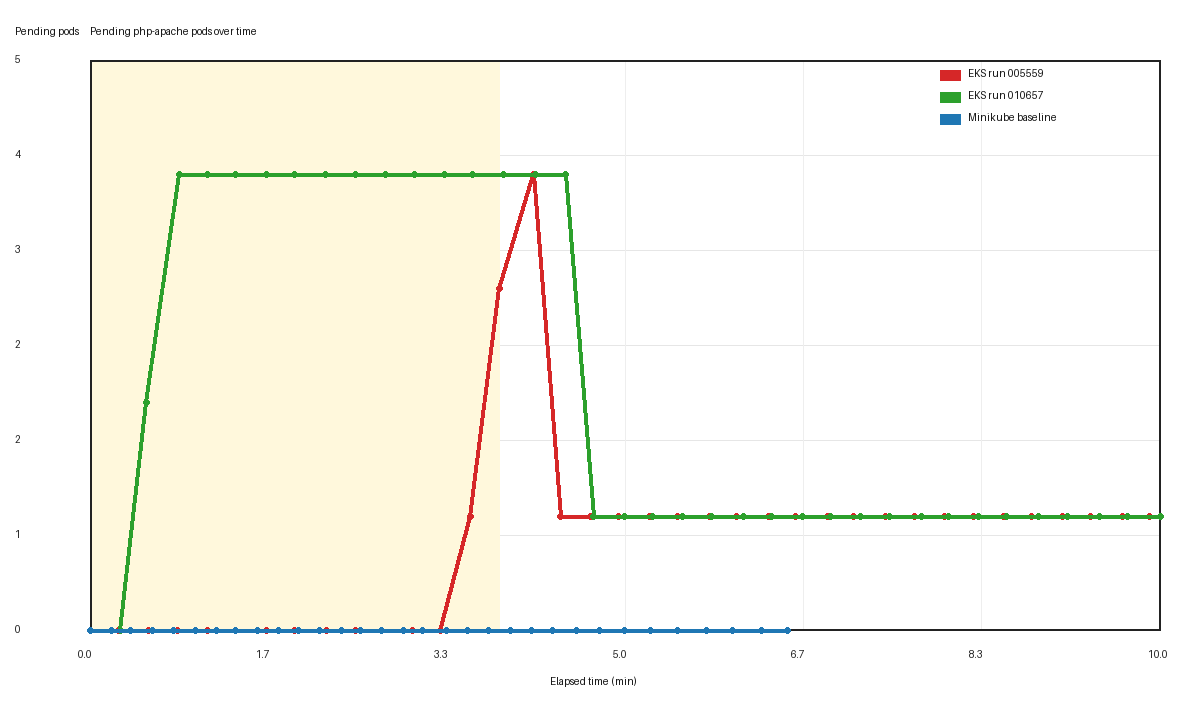
\includegraphics[width=\linewidth]{figures/baseline_pending_pods.png}
\caption{Pending workload pods over time. Pending pods appear in the EKS runs, but not in the Minikube baseline.}
\label{fig:baseline-pending-pods}
\end{figure}

The baseline also illustrates a measurement nuance. In Minikube, the HPA desired replica count eventually returned to 1 during the observation window, while the pod table could still show older pods during termination. The analysis therefore distinguishes HPA desired replicas from the instantaneous count of pod rows in \texttt{kubectl get pods}. In EKS, the more important distinction is between desired replicas and ready replicas: the HPA could raise the desired count, but several pods remained pending and did not contribute useful capacity.

\section{HPA Behavior-Tuning Extension}

The extension compares the default HPA behavior against two explicit \texttt{autoscaling/v2} policies: an aggressive scale-up policy and a faster scale-down policy. The expected trade-off is that faster scale-up may reduce the underprovisioning window, while faster scale-down may reduce replica-seconds after a burst but increase the risk of oscillation for intermittent workloads.

\begin{table}[ht]
\centering
\caption{Minikube HPA behavior-tuning comparison}
\label{tab:minikube-tuning}
\resizebox{\linewidth}{!}{%
\begin{tabular}{lrrrrr}
\toprule
Run & First scale-up (s) & Peak replicas & Pending pods & Scale-down after load (s) & Replica-s \\
\midrule
Minikube baseline rerun & 103 & 10 & 0 & 421 & 5581 \\
Minikube aggressive & 70 & 10 & 0 & 409 & 5560 \\
Minikube fast scale-down & 70 & 10 & 0 & 353 & 4149 \\
\bottomrule
\end{tabular}
}
\end{table}


\begin{figure}[ht]
\centering
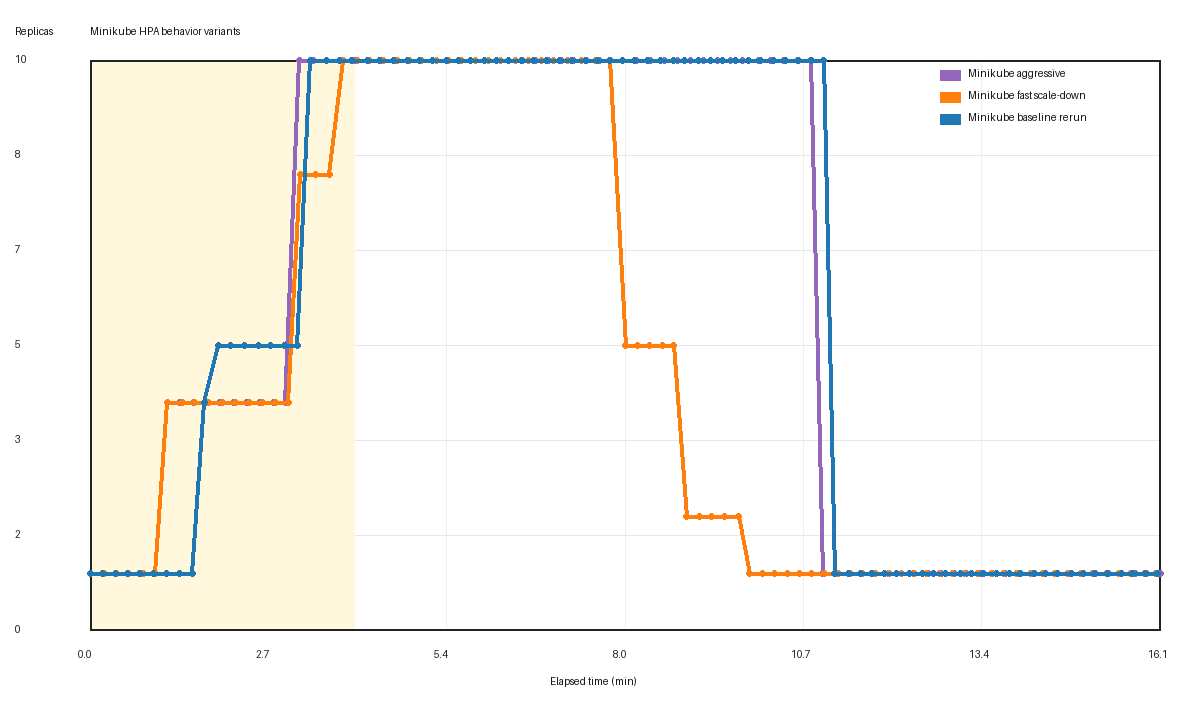
\includegraphics[width=\linewidth]{figures/minikube_hpa_tuning_replicas.png}
\caption{Desired replicas in the Minikube behavior-tuning runs. All runs used the same 240 s active-load window and 720 s post-load observation window.}
\label{fig:minikube-hpa-tuning}
\end{figure}

The comparable Minikube rerun shows that policy tuning changes the distribution of capacity over time even when all variants reach the same peak of 10 replicas. The aggressive policy reduced the first scale-up time from 103 s to 70 s and reached the peak slightly earlier, from 199 s to 189 s. However, its replica-second cost proxy remained nearly identical to the baseline rerun, because the scale-down behavior remained conservative. The fast scale-down policy preserved the same 70 s first scale-up time observed in the aggressive run, reduced scale-down after load removal from 421 s to 353 s, and lowered replica-seconds from 5581 to 4149. This represents a 25.7\% reduction in the replica-second proxy relative to the comparable baseline rerun.

This result is useful because it shows that HPA tuning should be evaluated against an explicit objective. If the objective is only to reduce reaction time, the aggressive policy helps. If the objective is to reduce excess capacity after bursts, the fast scale-down policy is more relevant. If the workload is intermittent, however, a shorter scale-down window may cause oscillation that is not visible in a single-burst experiment. For this reason, the observed 25.7\% reduction should be interpreted as a result for the tested burst shape, not as a universal recommendation.

\section{Cloud Infrastructure Constraints}

The EKS baseline is used to show the difference between configured elasticity and effective elasticity. HPA may set a higher desired replica count, but the scheduler can leave pods pending if nodes lack capacity. In the tested EKS configuration, \texttt{t3.micro} nodes are particularly constrained: the instance family is burstable, has limited memory, and, more importantly for this experiment, pod density is bounded by VPC CNI IP address capacity~\cite{aws_ec2_t3,aws_eks_vpc_cni}.

The VPC CNI documentation explains that, in the default mode, pod capacity depends on elastic network interfaces and IP addresses per interface~\cite{aws_eks_vpc_cni}. Therefore, the EKS cluster has a capacity dimension that does not exist in the same form in the single-node Minikube experiment. System pods also consume schedulable slots. In a small \texttt{t3.micro}-based node group, the practical capacity left for the workload and the load generators can be much smaller than the HPA \texttt{maxReplicas} value suggests.

This observation reframes the EKS result. It is not a failure of HPA; it is a boundary of pod-level autoscaling. The HPA controller can only change the replica field of the target Deployment. It cannot create EC2 instances, increase ENI limits, choose a larger instance type, or evict system pods. A production design that needs elastic capacity must combine HPA with a mechanism that scales the node pool, such as Cluster Autoscaler, Karpenter, or EKS Auto Mode~\cite{aws_eks_autoscaling}.

\begin{figure}[ht]
\centering
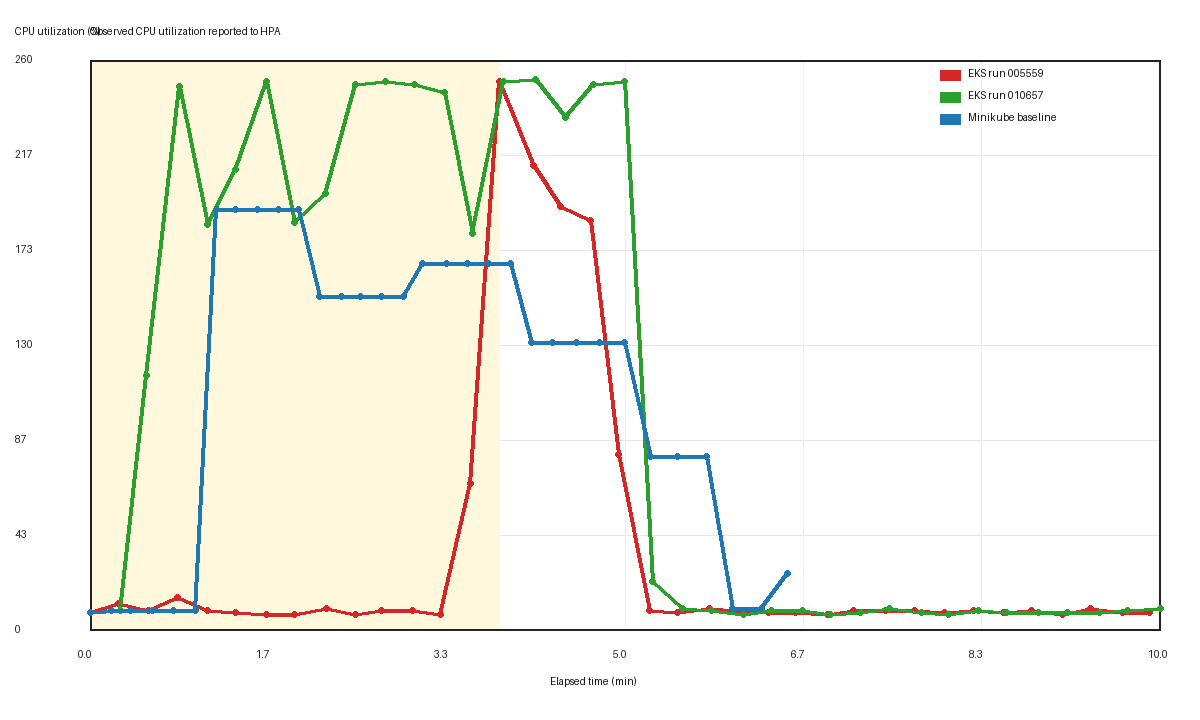
\includegraphics[width=\linewidth]{figures/baseline_cpu_utilization.png}
\caption{CPU utilization reported to HPA. EKS remains above target while workload pods are pending, showing that the desired replica count alone did not provide enough effective capacity.}
\label{fig:baseline-cpu}
\end{figure}

The practical diagnostic lesson is that HPA experiments should collect both autoscaler and scheduler evidence. The HPA table explains what the controller wanted. The pod table explains whether the scheduler could realize that decision. Node descriptions, daemonset placement, and pod events would be the next evidence layer when diagnosing a production incident.

\section{Cost and Operational Discussion}

Minikube has no direct cloud cost, but it depends on local host capacity and is not a production-grade managed environment. It is excellent for rapid iteration, YAML validation, and controlled single-node experiments. Its weakness is that local failures, host memory pressure, and virtualization issues become part of the experiment environment.

EKS introduces a managed control-plane charge and separate costs for worker nodes and related AWS resources~\cite{aws_eks_pricing}. In this project, the EKS experiment used a short-lived cluster and Free-Tier-constrained worker instances, so the absolute monetary cost was low. Still, the pricing model changes the engineering trade-off. Keeping extra replicas alive for longer has little direct cost in Minikube, but in a cloud cluster it consumes node resources that may require more or larger instances. If a Service of type \texttt{LoadBalancer} is used, cloud load balancer resources can also remain billable until explicitly removed.

\begin{table}[ht]
\centering
\caption{Cost components relevant to the EKS experiment}
\label{tab:cost-components}
\resizebox{\linewidth}{!}{%
\begin{tabular}{lll}
\toprule
Component & Pricing driver & Role in this project \\
\midrule
EKS control plane & Cluster-hour & Fixed cost while the cluster exists \\
EC2 worker nodes & Instance-hour & Capacity for workload and system pods \\
\texttt{t3.micro} nodes & US East Linux price & 2 vCPU, 1 GiB, burstable CPU credits \\
Load balancer & Resource-hour and traffic & Needed only for public external access \\
EBS and network & Volume, IP, traffic & Secondary costs for longer runs \\
\bottomrule
\end{tabular}
}
\end{table}

At the time of writing, AWS lists standard EKS cluster support at US\$0.10 per cluster-hour~\cite{aws_eks_pricing}. The EC2 T3 page lists \texttt{t3.micro} in US East (N. Virginia) with 2 vCPUs, 1.0 GiB of memory, 10\% baseline performance per vCPU, 12 CPU credits earned per hour, and an on-demand Linux price of US\$0.0104 per hour~\cite{aws_ec2_t3}. For the four-node EKS configuration used in the intermediate experiment, a simple compute-control-plane estimate is:

\begin{equation}
0.10 + 4 \times 0.0104 = 0.1416\ \mathrm{USD/hour},
\end{equation}

before load balancer, storage, public IPv4, data transfer, or tax effects. The numerical value is small for a short course experiment, but it illustrates why experiment cleanup is part of the methodology in cloud systems work.

The final tuning result should therefore be read through two cost lenses. At the application layer, replica-seconds estimate how much pod capacity is requested over time. At the infrastructure layer, node autoscaling and instance selection determine whether those requested replicas translate into additional cloud cost. A policy that reduces replica-seconds may lower waste only if the cluster can consolidate or release nodes. Without node autoscaling, the nodes remain allocated even if HPA scales the application back down.

Operationally, the most robust architecture would treat HPA as one control loop among several. HPA controls replicas. Cluster Autoscaler or Karpenter controls nodes. Metrics Server supplies the resource metrics needed by HPA. Prometheus or another observability stack should supply historical analysis. IAM, VPC, CNI, and instance-type choices define the capacity envelope in EKS. The course experiment is small, but it exposes the same decomposition needed in real deployments.

\section{Design Implications}

The first design implication is that \texttt{maxReplicas} is not a capacity guarantee. It is only an upper bound on the desired replica count that HPA may write to the target workload. In Minikube, this distinction is less visible because the cluster is single-node and unconstrained by cloud networking quotas. In EKS, the distinction appears immediately: desired replicas can exceed effective schedulable capacity.

The second implication is that CPU-only autoscaling is easy to reproduce but limited as an application policy. It is appropriate for the selected workload because the endpoint intentionally burns CPU. It would be less appropriate for a request-driven service bottlenecked by downstream latency, database connections, queue depth, memory pressure, or external API limits. In those cases, resource metrics should be complemented by custom or external metrics. Kubernetes supports these metric classes through separate metrics APIs~\cite{kubernetes_hpa_concepts}, but each additional metric source also increases operational complexity.

The third implication is that scale-down policy deserves as much attention as scale-up policy. Most classroom demonstrations emphasize the visible moment when replicas increase. The cost and stability questions often appear after the burst, when the system decides how long to keep spare capacity. The tuning runs show this directly: the fast scale-down policy had the same peak as the baseline and aggressive runs, but substantially fewer replica-seconds.

The fourth implication is that node autoscaling is the natural complement to HPA in managed cloud environments. If HPA creates pending pods and the application remains above target, the next question is not another HPA parameter; it is whether the cluster can add nodes or choose larger nodes. This is where Cluster Autoscaler, Karpenter, or EKS Auto Mode become relevant~\cite{aws_eks_autoscaling}.

\section{Operational Lessons}

The experiment produced three operational lessons that are useful beyond the numerical results. First, raw evidence should include both controller state and pod state. A log containing only \texttt{kubectl get hpa} would show desired replicas, but it would not reveal whether pods were pending. A log containing only pod state would miss the controller's recommendation. The combination makes the diagnosis possible.

Second, the observation window must match the controller behavior being studied. A short post-load window can miss scale-down completely, especially under the default 300 s stabilization window. The final reruns used a 720 s post-load window to avoid interpreting missing data as missing behavior.

Third, the local environment is itself an experimental variable. During the final runs, the Minikube profile had to be restarted after a KVM/libvirt networking issue. This did not affect the completed logs, but it reinforces the need to keep setup scripts, cleanup scripts, and raw evidence together. Reproducibility in cloud computing courses is not only about application code; it also depends on documenting the infrastructure path.

\section{Future Work}

The most direct next experiment is HPA plus node autoscaling in EKS. The experimental sequence would be: start with limited node capacity, generate CPU load, let HPA create additional desired replicas, observe pending pods, allow Karpenter or Cluster Autoscaler to provision nodes, and measure the time until the new pods become ready. This would quantify the full elasticity path from application demand to cloud infrastructure allocation.

A second extension is to replace the synthetic CPU-bound endpoint with a small service exposing multiple bottleneck modes: CPU-bound, memory-bound, latency-bound, and queue-backed. This would allow a direct comparison between CPU utilization, memory utilization, custom metrics, and external metrics. It would also make it possible to show cases where CPU-based HPA reacts too late or reacts to the wrong signal.

A third extension is observability. Metrics Server is enough for HPA, but it is not designed as a historical monitoring system~\cite{kubernetes_metrics_server}. A Prometheus-based setup could collect higher-resolution time series for CPU, memory, request rate, request latency, replica count, and node pressure. That would enable stronger plots and statistical comparisons across repeated runs.

A final extension is cost-aware autoscaling. The replica-second proxy used here is intentionally simple. A more complete study would combine replica-seconds, node-hours, load balancer hours, and request-level service metrics to estimate the trade-off between cost, response time, and stability. That extension would move the work closer to production capacity planning.

\section{Threats to Validity}

The workload is intentionally simple and CPU-bound, so results should not be generalized to all microservice or I/O-bound systems. The benefit is controllability: CPU pressure is easy to generate and is directly connected to the HPA target. The limitation is that real applications may bottleneck on memory, network, disk, database connections, queue depth, or tail latency before CPU becomes the dominant signal.

The EKS experiment used small Free-Tier-constrained instances, which makes infrastructure constraints visible but does not represent all production EKS clusters. Larger instances, prefix delegation, different CNI settings, Fargate, Karpenter, or EKS Auto Mode could change the effective capacity boundary. The conclusion is therefore not that EKS is less capable than Minikube; it is that managed cloud clusters have additional capacity dimensions that must be configured intentionally.

The final Minikube tuning experiment used one run per policy after a comparable baseline rerun. That is enough to support an educational comparison, but not enough for statistical inference. Future repetitions should execute each policy multiple times, randomize run order, and report variability. A richer experiment would also add request latency, throughput, and node-level CPU metrics.

Finally, Metrics Server values are sufficient for HPA control but are not a high-resolution observability dataset. The parser preserves the control-plane evidence available through \texttt{kubectl}, but it cannot reconstruct every request or scheduling decision. This limitation is acceptable for the stated research questions, which focus on autoscaling behavior rather than application benchmarking.

\section{Conclusion}

This final project extends a working HPA comparison into a broader empirical study of Kubernetes elasticity. The baseline results show that the same HPA policy can reach the configured maximum in Minikube while being capped below that maximum in EKS by schedulable capacity. The tuning results show that explicit \texttt{autoscaling/v2} behavior policies can materially change the capacity profile over time: in the comparable Minikube runs, the fast scale-down policy reduced replica-seconds by 25.7\% relative to the baseline rerun.

The main conclusion is that HPA is necessary but insufficient. Practical autoscaling requires aligning application metrics, resource requests, controller behavior, schedulable capacity, node autoscaling, networking limits, and cloud cost. For future work, the most valuable next experiment would combine HPA with node autoscaling in EKS and measure the full delay from load increase to newly provisioned nodes running useful application pods.

\bibliographystyle{IEEEtran}
\bibliography{references}

\end{document}
